%%%------------------------------------------------------------------------------------------------------------
%%% 调序模型1:基于距离的调序
\begin{center}
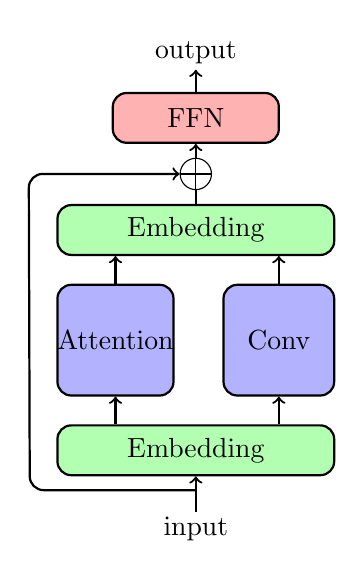
\begin{tikzpicture}

\tikzstyle{manode}=[rectangle,inner sep=0mm,minimum height=4em,minimum width=4em,rounded corners=5pt,thick,draw,fill=blue!30]
\tikzstyle{ffnnode}=[rectangle,inner sep=0mm,minimum height=1.8em,minimum width=6em,rounded corners=5pt,thick,fill=red!30,draw]
\tikzstyle{ebnode}=[rectangle,inner sep=0mm,minimum height=1.8em,minimum width=10em,rounded corners=5pt,thick,fill=green!30,draw]

\begin{scope}[]

\node [anchor=west,inner sep=0mm,minimum height=1.8em] (f1) at (0, 0){input};
\node [anchor=south,ebnode] (e1) at ([xshift=0em,yshift=1em]f1.north){Embedding};
\node [anchor=south west,manode] (a1) at ([xshift=0em,yshift=1em]e1.north west){Attention};
\node [anchor=south east,manode] (c1) at ([xshift=0em,yshift=1em]e1.north east){Conv};
\node [anchor=south west,ebnode] (e2) at ([xshift=0em,yshift=1em]a1.north west){Embedding};
\node [anchor=south,draw,circle,inner sep=4pt] (add1) at ([xshift=0em,yshift=0.5em]e2.north){};
\node [anchor=south,ffnnode] (f2) at ([xshift=0em,yshift=0.5em]add1.north){FFN};
\node [anchor=south,inner sep=0mm,minimum height=1.8em] (op) at ([xshift=0em,yshift=0.5em]f2.north){output};


\draw[->,thick] ([xshift=0em,yshift=-0.3em]f1.north)--([xshift=0em,yshift=0em]e1.south);
\draw[->,thick] ([xshift=0em,yshift=-1em]a1.south)--([xshift=0em,yshift=0em]a1.south);
\draw[->,thick] ([xshift=0em,yshift=-1em]c1.south)--([xshift=0em,yshift=0em]c1.south);
\draw[->,thick] ([xshift=0em,yshift=0em]a1.north)--([xshift=0em,yshift=1em]a1.north);
\draw[->,thick] ([xshift=0em,yshift=0em]c1.north)--([xshift=0em,yshift=1em]c1.north);
\draw[-,thick] ([xshift=0em,yshift=0em]e2.north)--([xshift=0em,yshift=0em]add1.south);
\draw[->,thick] ([xshift=0em,yshift=0em]add1.north)--([xshift=0em,yshift=0em]f2.south);
\draw[->,thick] ([xshift=0em,yshift=0em]f2.north)--([xshift=0em,yshift=0.3em]op.south);


\draw[-] ([xshift=0em,yshift=0em]add1.west)--([xshift=-0em,yshift=0em]add1.east);
\draw[-] ([xshift=0em,yshift=0em]add1.south)--([xshift=-0em,yshift=-0em]add1.north);


\draw[->,thick,rectangle,rounded corners=5pt] ([xshift=0em,yshift=0.5em]f1.north)--([xshift=-6em,yshift=0.5em]f1.north)--([xshift=-5.45em,yshift=0em]add1.west)--([xshift=0em,yshift=0em]add1.west);


\end{scope}
\end{tikzpicture}
\end{center}